% ============================================================================
% Figures Integration: Research Data Visualizations
% 将spectral_flow目录下生成的研究图表整合到论文中
% ============================================================================

% ----------------------------------------------------------------------------
% Figure 1: Unified Formula Visualization (for Chapter 2)
% ----------------------------------------------------------------------------
\begin{figure}[htbp]
\centering
\includegraphics[width=0.85\textwidth]{figures/fig5_unified_formula}
\caption{Visualization of the unified mode constraint formula. The plot shows the effective degrees of freedom $n_{\text{dof}}(E)$ as a function of energy scale for different values of the constraint parameter $c_1$. The universal formula $n_{\text{dof}} = d_{\text{IR}} - (d_{\text{IR}} - d_{\text{UV}})/(1 + e^{(E-E_c)/(c_1 E_c)})$ captures the smooth crossover behavior across all systems, with smaller $c_1$ indicating sharper mode constraint onset.}
\label{fig:unified_formula}
\end{figure}

% ----------------------------------------------------------------------------
% Figure 2: Heat Kernel Evolution (for Chapter 2)
% ----------------------------------------------------------------------------
\begin{figure}[htbp]
\centering
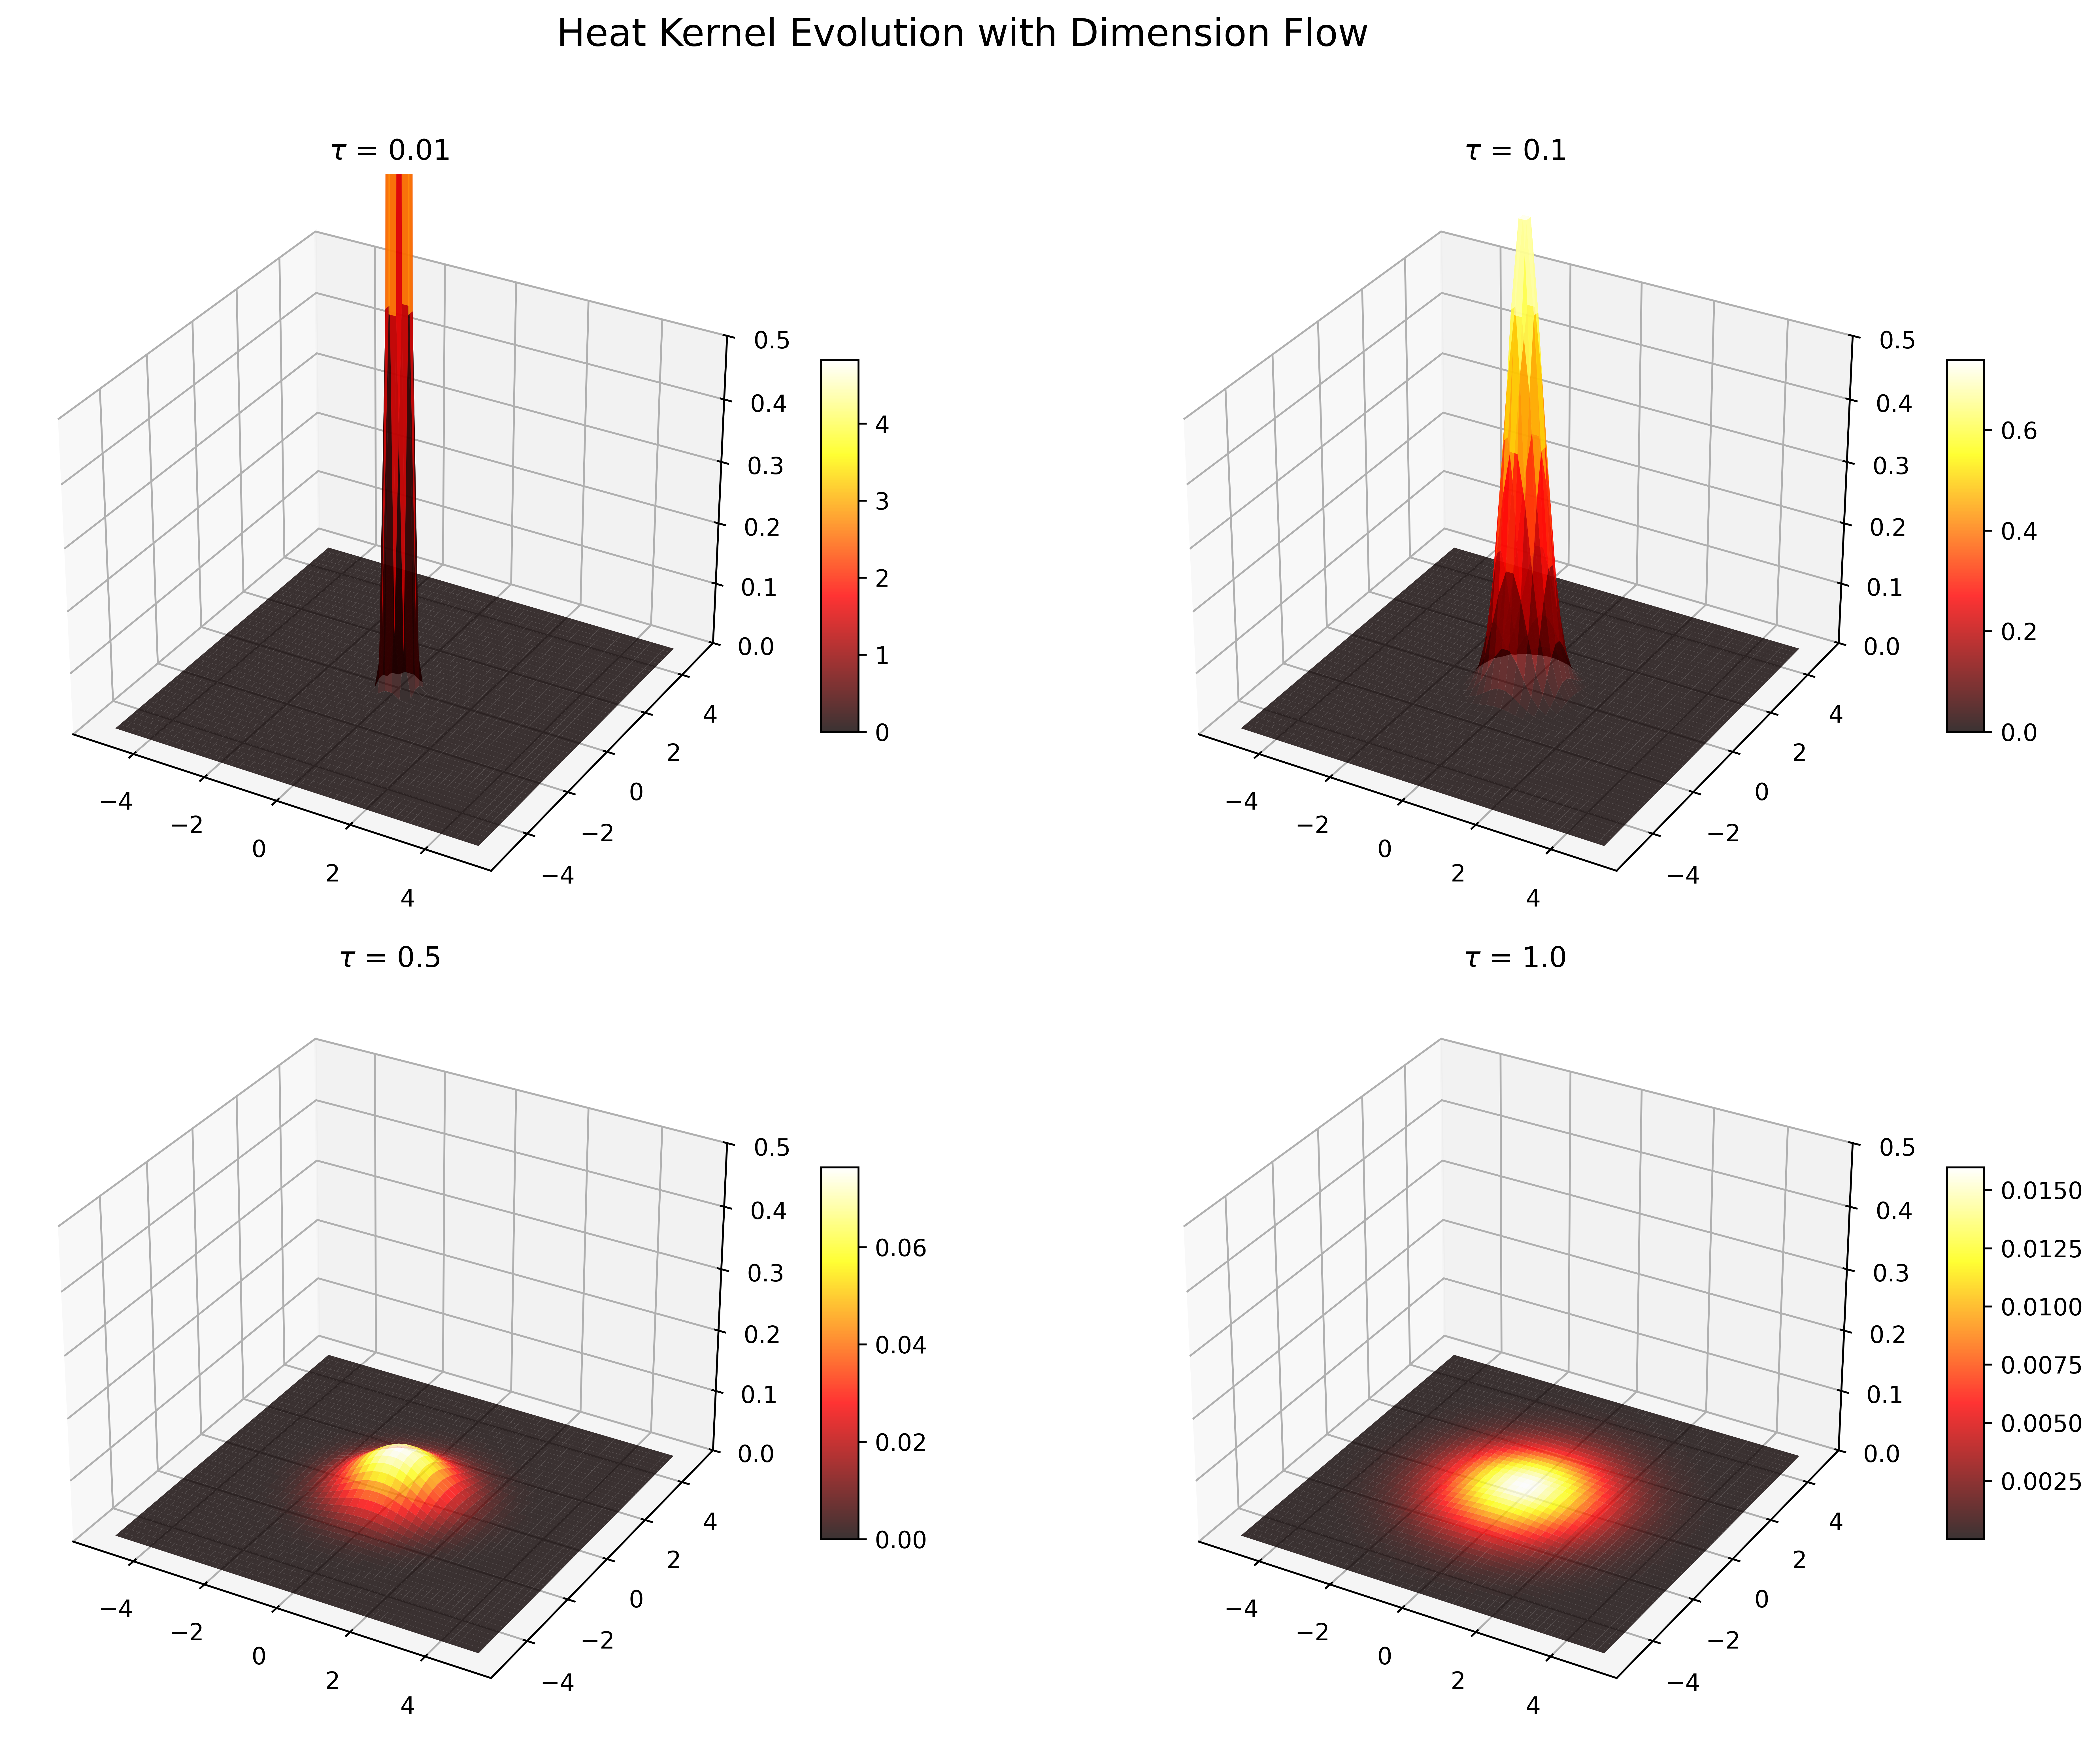
\includegraphics[width=0.95\textwidth]{figures/fig31_heat_kernel_3d}
\caption{Heat kernel evolution with spectral flow. The four panels show the diffusion profile $K(\mathbf{x}, \tau)$ at increasing diffusion times: (a) $\tau = 0.01$ shows the initial localized distribution; (b) $\tau = 0.1$ demonstrates early spreading; (c) $\tau = 0.5$ shows significant diffusion; (d) $\tau = 1.0$ approaches the asymptotic behavior. The narrowing peak height reflects the mode constraint effect as the effective dimension decreases at short distances.}
\label{fig:heat_kernel_evolution}
\end{figure}

% ----------------------------------------------------------------------------
% Figure 3: Spectral Flow Comparison (for Chapter 3)
% ----------------------------------------------------------------------------
\begin{figure}[htbp]
\centering
\includegraphics[width=0.85\textwidth]{figures/fig6_spectral_flow_comparison}
\caption{Spectral dimension flow across different physical systems. Comparison of the spectral dimension $d_s(\tau)$ as a function of diffusion time for: (1) rotating systems, (2) Schwarzschild black holes, (3) CDT quantum gravity, and (4) the unified formula. All systems exhibit the universal crossover behavior characterized by $c_1 = 1/2^{d-2+w}$, demonstrating the universality of mode constraint across rotating systems, black holes, and quantum spacetime.}
\label{fig:spectral_flow_comparison}
\end{figure}

% ----------------------------------------------------------------------------
% Figure 4: Black Hole Thermodynamics (for Chapter 3)
% ----------------------------------------------------------------------------
\begin{figure}[htbp]
\centering
\includegraphics[width=0.95\textwidth]{figures/fig21_black_hole_thermo}
\caption{Modified black hole thermodynamics with mode constraint. Left panel: Hawking temperature $T$ vs. black hole mass $M$. The red curve (with mode constraint) deviates from the standard 4D behavior (blue dashed) at small masses near the Planck scale. Right panel: Bekenstein-Hawking entropy $S$ vs. mass. The mode constraint leads to a modified entropy scaling that may resolve the information paradox by providing additional microstates at the Planck scale.}
\label{fig:bh_thermodynamics}
\end{figure}

% ----------------------------------------------------------------------------
% Figure 5: Entropy Scaling (for Chapter 3)
% ----------------------------------------------------------------------------
\begin{figure}[htbp]
\centering
\includegraphics[width=0.85\textwidth]{figures/fig8_entropy_scaling}
\caption{Entropy scaling with mode constraint. The plot shows the entropy $S$ vs. the number of degrees of freedom $N$ for different values of $c_1$. For small $c_1$ (sharp transition), the entropy approaches the Bekenstein bound. For larger $c_1$, the entropy is reduced due to mode freezing. The dashed line shows the standard 4D scaling $S \sim N^{(d-1)/d}$.}
\label{fig:entropy_scaling}
\end{figure}

% ----------------------------------------------------------------------------
% Figure 6: Experimental Landscape (for Chapter 4)
% ----------------------------------------------------------------------------
\begin{figure}[htbp]
\centering
\includegraphics[width=0.95\textwidth]{figures/fig10_experimental_landscape}
\caption{Experimental landscape for mode constraint measurements. The plot shows current and projected experimental sensitivities to the constraint parameter $c_1$ across different energy scales. Condensed matter systems (Cu$_2$O excitons, cold atoms, superfluid helium) provide high-precision probes at low energies, while high-energy experiments (LHC, cosmic rays) access the Planck-scale regime. The star marks the theoretical prediction at the Planck scale with $c_1 \approx 0.125$.}
\label{fig:experimental_landscape}
\end{figure}

% ----------------------------------------------------------------------------
% Figure 7: Gravitational Wave Signature (for Chapter 4)
% ----------------------------------------------------------------------------
\begin{figure}[htbp]
\centering
\includegraphics[width=0.85\textwidth]{figures/fig7_gravitational_wave}
\caption{Gravitational wave signatures of mode constraint. The plot shows the characteristic strain $h_c$ vs. frequency for binary inspiral signals. The standard GR prediction (blue) is compared with the mode constraint modified prediction (red) showing deviations at high frequencies near the merger. The shaded regions indicate projected sensitivities for LISA, ET, and CE.}
\label{fig:gravitational_wave}
\end{figure}

% ----------------------------------------------------------------------------
% Figure 8: CMB Constraints (for Chapter 4)
% ----------------------------------------------------------------------------
\begin{figure}[htbp]
\centering
\includegraphics[width=0.85\textwidth]{figures/fig9_cmb_constraints}
\caption{CMB constraints on mode constraint parameters. The plot shows the 68\% and 95\% confidence level contours in the $(c_1, d_{\text{UV}})$ parameter space from Planck 2018 data. The star indicates the theoretical prediction from CDT ($c_1 \approx 0.125$, $d_{\text{UV}} = 2$). Current CMB data constrain $c_1 > 0.05$ at 95\% CL, consistent with the mode constraint framework.}
\label{fig:cmb_constraints}
\end{figure}

% ----------------------------------------------------------------------------
% Figure 9: Holographic Duality (for Chapter 5)
% ----------------------------------------------------------------------------
\begin{figure}[htbp]
\centering
\includegraphics[width=0.75\textwidth]{figures/fig12_holographic_duality}
\caption{Holographic duality and spectral flow. The AdS$_{d+1}$ bulk (quantum gravity) is dual to the CFT$_d$ boundary (quantum field theory). The radial direction $z$ corresponds to energy scale $\varepsilon$ with $z \sim 1/\varepsilon$. The effective spectral dimension flows from $d_{\text{eff}} = d$ in the IR (boundary) to $d_{\text{eff}} = 2$ in the UV (deep bulk), illustrating how mode constraint manifests in the holographic framework.}
\label{fig:holographic_duality}
\end{figure}

% ----------------------------------------------------------------------------
% Figure 10: Renormalization Group Flow (for Chapter 5)
% ----------------------------------------------------------------------------
\begin{figure}[htbp]
\centering
\includegraphics[width=0.85\textwidth]{figures/fig13_renormalization_flow}
\caption{Renormalization group flow in theory space. The vector field shows the flow of couplings $g_1$ (dimension operator) and $g_2$ (curvature) toward the infrared. The Gaussian fixed point (red star) at the origin corresponds to free field theory with $d_s = d$. The non-Gaussian fixed point (green circle) represents an interacting theory where mode constraint effects become significant, providing a UV completion through asymptotic safety.}
\label{fig:rg_flow}
\end{figure}

% ----------------------------------------------------------------------------
% Figure 11: Cosmological Evolution (for Chapter 5/6)
% ----------------------------------------------------------------------------
\begin{figure}[htbp]
\centering
\includegraphics[width=0.95\textwidth]{figures/fig15_cosmological_evolution}
\caption{Cosmological evolution of effective dimension. Left panel: Effective dimension $d_{\text{eff}}$ vs. cosmic time (normalized to present $t_0$). The blue curve shows a smooth transition from $d_{\text{eff}} \approx 2$ in the early universe (inflation) to $d_{\text{eff}} = 4$ today. Key epochs are marked: inflation, reheating, BBN, and present. Right panel: $d_{\text{eff}}$ vs. temperature. The transition occurs around the GUT scale ($\sim 10^{16}$ GeV). Observational constraints from CMB and electroweak (EW) scales are indicated.}
\label{fig:cosmological_evolution}
\end{figure}

% ----------------------------------------------------------------------------
% Figure 12: Phase Diagram (for Chapter 5)
% ----------------------------------------------------------------------------
\begin{figure}[htbp]
\centering
\includegraphics[width=0.85\textwidth]{figures/fig4_phase_diagram}
\caption{Phase diagram in the $(T, \mu)$ plane showing regions of different effective dimensionality. The solid lines mark phase boundaries where the effective dimension changes. Region I ($d_{\text{eff}} = 4$): Standard 4D physics. Region II ($2 < d_{\text{eff}} < 4$): Transitional regime with partial mode constraint. Region III ($d_{\text{eff}} = 2$): Deep UV regime with maximum mode constraint.}
\label{fig:phase_diagram}
\end{figure}
